\subsection{E-step versus sleep phase}
\label{sec:estep_sleep_compare}

In this subsection, we compare the posteriors obtained by optimizing the sleep phase objective~\eqref{eq:sleep_phase_summary} 
versus optimizing the E-step objective~\eqref{eq:e_step}, also known as the ELBO. 
We demonstrate on a toy example that there exist shallow optima in the ELBO where the variational posterior on locations does not concentrate around the true locations.
We show that the sleep phase objective is able to avoid these shallow optima. 
We use simulated data with known PSF and background for this example, so the wake-phase (M-step) is not needed. 

In this toy example, we simulated a $20\times20$ single-band image, shown in Figure~\ref{fig:toy_example}.
The image has four stars, each with the same flux. It is divided into four $10\times 10$ tiles, which are the inputs to the neural network. The image, call it $x_{test}$, was fixed for this experiment. 

\begin{figure}[!h]
    \centering
    \vspace{-1em}
    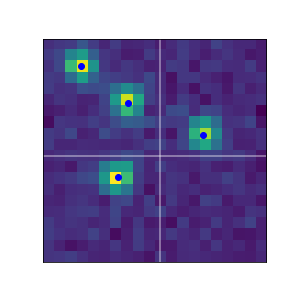
\includegraphics[width = 0.3\textwidth]{figures/vi_sleep_ex_figure.png}
    \vspace{-1.7em}
    \caption{The example $20\times 20$ image with four stars. The outlined $10\times 10$ tiles are inputs to the neural network. }
    \label{fig:toy_example}
\end{figure}

In our generative model, we set the prior on the number of stars $N$ to be Poisson with mean $\mu = 4$ and the prior on flux to have a power law slope $\alpha = 0.5$. 
With these these prior parameters, we compare directly optimizing the ELBO, 
\begin{align}
\Expect_{q_{\eta}(z | x_{test})}\Big[\log p(x_{test}, z) - \log q_{\eta}(z | x_{test})\Big],
\label{eq:elbo_on_test}
\end{align}
against optimizing the sleep phase objective. Note that optimizing the sleep phase does not depend on $x_{test}$; it only requires drawing catalogs from the aforementioned prior and simulated images given the catalog. 


In Figure~\ref{fig:optim_path} (top row), we display the ELBO~\eqref{eq:elbo_on_test} as the optimization proceeds.
In the left-most plot, we optimized the ELBO using stochastic gradient descent with the REINFORCE estimator.
The optimization did not converge, likely due to the high variance of the REINFORCE estimator. 
In the middle plot, we analytically integrated the ELBO with respect to the variational distribution on the number of stars $N$ before computing stochastic gradients using the reparameterization trick.
See Appendix TBD for details about the gradient estimators. 
The reparameterized gradients exhibited lower variance, and the optimization was able to converge to stationary points. 
However, depending on the initialization, the variational distribution converged to points where the ELBO is non-optimal (e.g. restarts 3 and 6). 
In contrast, optimizing the sleep phase consistently converged to a similar ELBO across all restarts. 

In the bottom left of Figure~\ref{fig:optim_path}, we display the MAP locations found after getting stuck in a local minima. In the tile with two stars, both MAP locations were placed on one star. Ideally, one of the locations would be shifted to the second star. However, to move one location to the second star, the optimization path must traverse a region where the log-likelihood is lower than the current configuration. The displayed configuration is a local optima where the gradient with respect to its locations is approximately zero. In contrast, the sleep phase optimization consistently placed MAP locations around the four true stars. An example using the first restart is shown. 

\begin{figure}[!htb]
    \centering
    \begin{subfigure}[t]{0.9\textwidth}
    \centering
    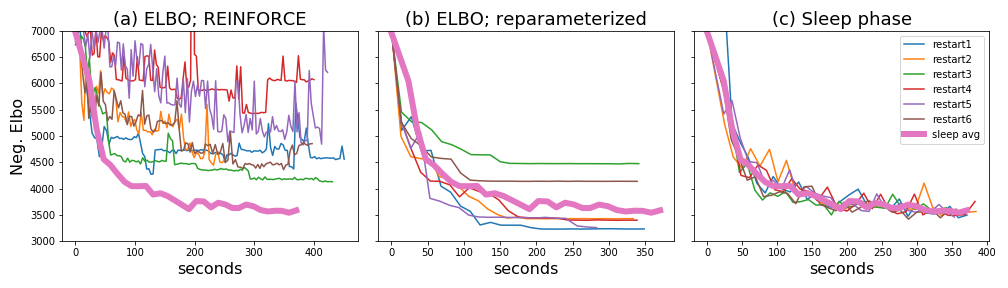
\includegraphics[width=\textwidth]{figures/optim_path_compare.png}
    \end{subfigure}
    \begin{subfigure}[t]{\textwidth}
    \centering
    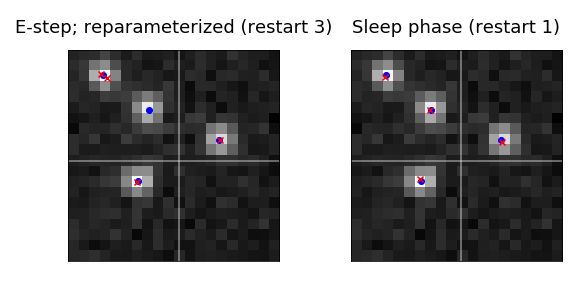
\includegraphics[width=0.55\textwidth]{figures/optim_path_detect_compare.png}
    \end{subfigure}
    \vspace{-3em}
    \caption{(Top) The ELBO as the optimization progresses, for six random restarts. Bold pink line in all plots is the sleep phase ELBO path, averaged over six restarts. (Bottom) MAP locations from two variational posteriors shown in red. On the left, the detections from restart 3 of using the reparameterized gradient, where the optimization got stuck in local optima. All posteriors optimized with the sleep phase posteriors correctly detected four stars. Restart 1 is shown on the right. }
    \label{fig:optim_path}
\end{figure}

Figure~\ref{fig:gradzero_cartoon} shows schematic of this general phenomenon. When the estimated location is far from the true location, the gradient of the ELBO with respect to location vanishes. Because the PSF is nearly zero everywhere except for a few pixels around each location, a small shift in location does not significantly change the likelihood unless the estimated location is within a ``PSF radius" of the true location. On the other hand, the sleep phase objective is quadratic in the estimated location -- see~\eqref{eq:gaussian_sleep_loss}. Thus, the further the estimated location from the true location, the larger the gradient. The gradient does not vanish in the sleep phase objective. 

\begin{figure}[!htb]
    \centering
    \begin{subfigure}[t]{0.8\textwidth}
    \centering
    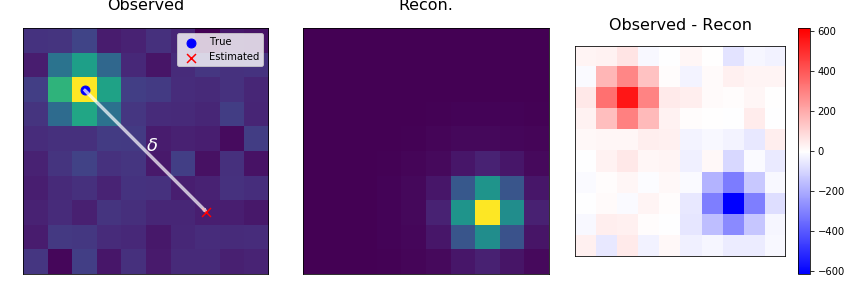
\includegraphics[width=\textwidth]{figures/gradzero_cartoon.png}
    \end{subfigure}
    \begin{subfigure}[t]{\textwidth}
    \centering
    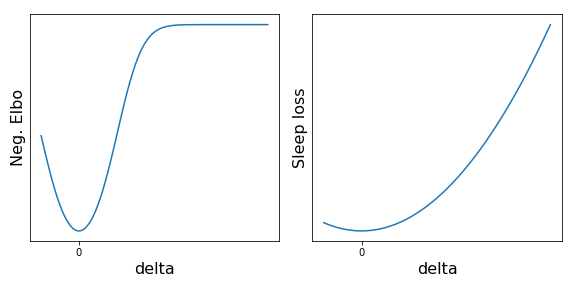
\includegraphics[width=0.55\textwidth]{figures/gradzero_cartoon2.png}
    \end{subfigure}
    \vspace{-3em}
    \caption{A cartoon illustration of vanishing gradients. Because the estimated star is far from the true star, the log-likelihood (and relatedly the ELBO) does not change for any location in an $\epsilon$ ball of the estimated location. 
    For large delta, the gradient of the ELBO is with respect to locations is zero. In contrast, the sleep phase loss is quadratic in the estimated location, and the gradient does not vanish. }
    \label{fig:gradzero_cartoon}
\end{figure}

Also note that we required analytically integrating out $N$ on this toy example in order to construct low-variance gradients. 
In this example, we set $N_{max}$ on each tile to be two; in other words, the neural network infers either 0, 1, or 2 stars on each tile.
Since the variational distribution factorizes over the four tiles, integrating $N$ is a summation of $3^4 = 81$ terms.
On larger images with more tiles, analytically integrating $N$ would be computationally infeasible, and REINFORCE gradients would be required. 

To illustrate on a larger example, Figure~\ref{fig:sim_data100x100} displays our results on a simulated $100\times 100$ image with fifty stars. The tiles again consisted of $10\times 10$ pixels. Optimizing the sleep phase objective resulted in near perfect in estimation of locations; optimizing the ELBO appears to be hindered by regions with little gradient information and is slow to converge. 

\begin{figure}[!htb]
    \centering
    \begin{subfigure}[!t]{0.4\textwidth}
    \centering
    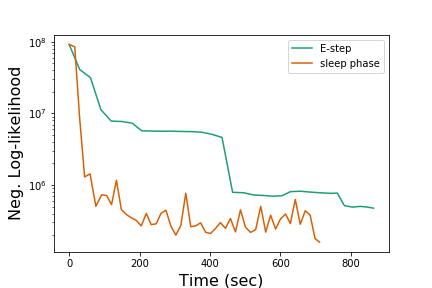
\includegraphics[width=\textwidth]{figures/optim_path_compare_100x100.png}
    \end{subfigure}
    \begin{subfigure}[!t]{0.59\textwidth}
    \centering
    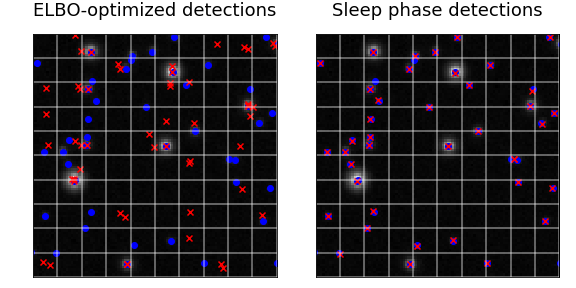
\includegraphics[width=\textwidth]{figures/optim_path_detect_compare_100x100.png}
    \end{subfigure}
    \caption{(Left) The log-likelihoood evaluated at the MAP estimate under the variational posterior. (Right) Detections on the a $100\times 100$ image, with true stars in blue, and MAP locations in red. TODO: fix the colors of this plot ... same issue with sparse field plot later.}
    \label{fig:sim_data100x100}
\end{figure}
